\chapter{LuaJIT overview}

This chapter aims to present an overview of LuaJIT. The first paragraph outlines the Lua programming language, then the following paragraphs focus on LuaJIT architecture, virtual machine (VM) and just-in-time compiler (JIT).

\section{Lua}
Lua is described on its official website \cite{lua-programming} as a powerful, efficient, lightweight, embeddable scripting language. It supports procedural programming, object-oriented programming, functional programming, data-driven programming, and data description. It is designed, implemented, and maintained by a team at PUC-Rio, the Pontifical Catholic University of Rio de Janeiro in Brazil.
 
Lua combines simple procedural syntax with powerful data description constructs based on associative arrays and extensible semantics. Lua runs by interpreting bytecode with a register-based virtual machine. It is dynamically typed and has automatic memory management with incremental garbage collection.

Lua is specifically known for its performance. Experiments on several benchmarks show Lua as one the fastest interpreted scripting languages ever made.

\section{LuaJIT}
LuaJIT \cite{pall2012luajit} is a trace-based 
just-in-time compiler for the Lua programing language. It is widely considered to be one of the fastest dynamic language implementations as it outperforms other dynamic languages on many cross-language benchmarks.
In this paragraph, we will go through a description of its internal architecture, which is shown in Fig. \ref{fig:schematic-luajit}.
 
\begin{figure}[H]
    \centering
	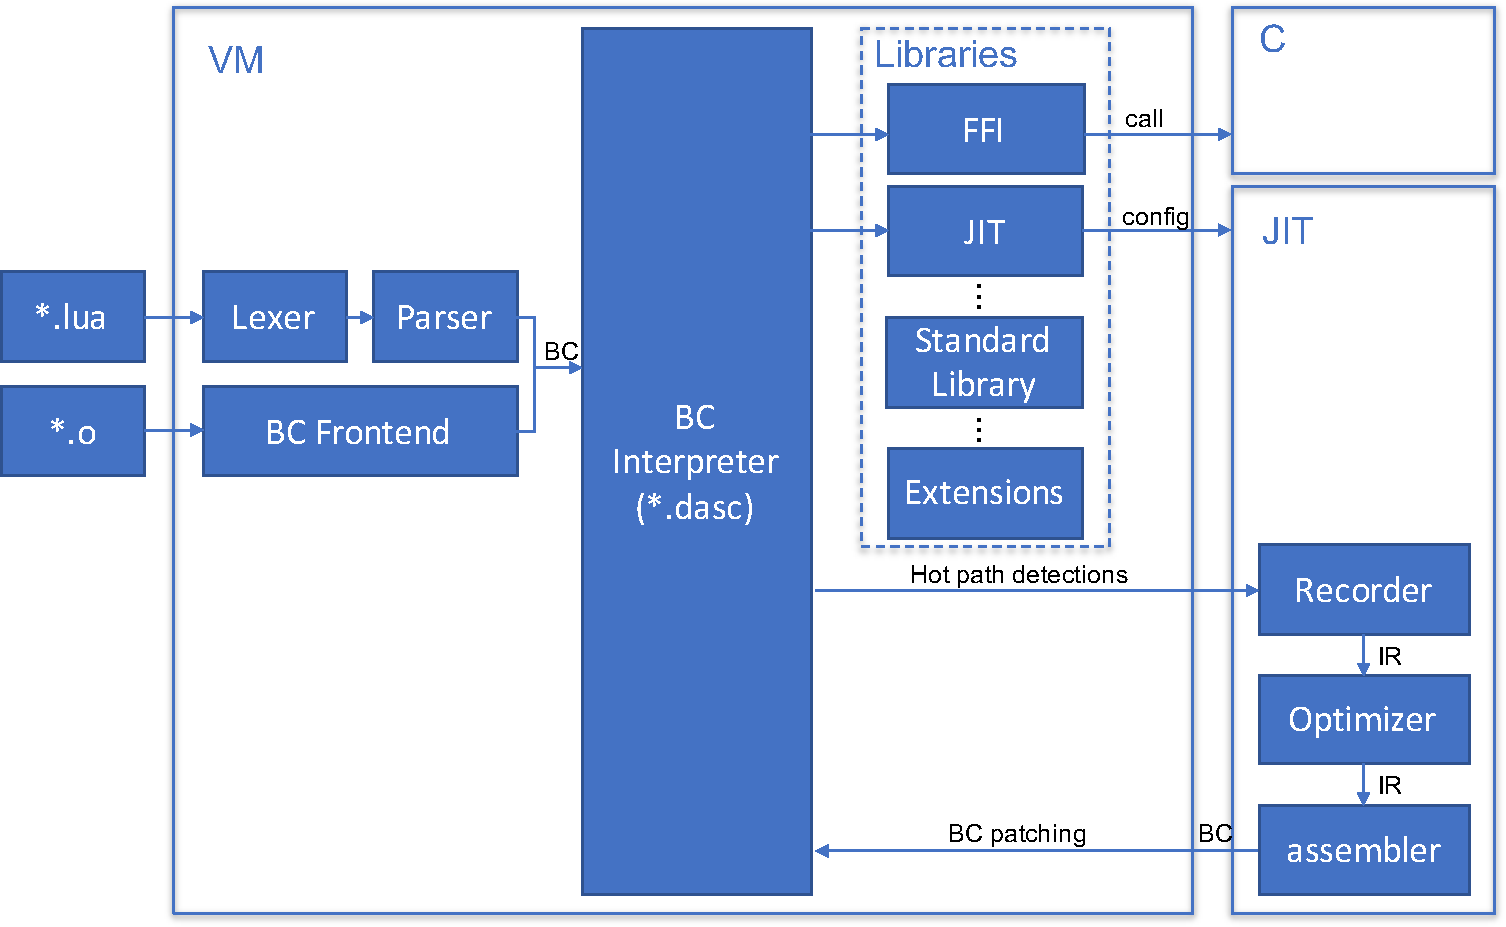
\includegraphics[width=\textwidth]{images/chapter1/LuaJIT-schematic.pdf}
    \caption{Schematic view of LuaJIT internals (source \cite{bloch2018madng})}
    \label{fig:schematic-luajit}
\end{figure}

\noindent
The compiler fronted is represented by the blocks \textit{Lexer}, \textit{Parser} and \textit{BC Frontend}. The input can either be text files containing Lua code (\texttt{*.lua}) or object files (\texttt{*.o}). Lua files are processed by \textit{Lexer} and \textit{Parser} that generate LuaJIT bytecode instructions (BC). On the other hand, object files, which contain already converted LuaJIT bytecode instructions, are read by the \textit{BC Frontend}. 

Once the source code is translated to bytecode instructions, the \textit{BC interpreter} executes them. The interpreter of LuaJIT is fully written in assembly (files \texttt{*.dasc}). It performs very fast interpretation and it uses DynASM \cite{pall2012dynasm} as a powerful cross-platform assembler. 

Several libraries are used to support the \textit{BC interpreter} in its tasks. Within these library the most relevants are: (i) the foreign function interface (\textit{FFI}) which allows to inject C code into Lua in a very efficient way; (ii) the \textit{Standard Library} to manipulate Lua data (stack, registry, etc.); (iii) the \textit{JIT} library that provides the functions to configure the JIT engine; (iv) the \textit{Extentions} of Lua.

The core of LuaJIT is represented by the JIT engine. LuaJIT detects hotpaths from frequently executed fragments of code. Once a hotpath is detected, the executed bytecode instructions are recorded into a trace by the \textit{Recorder} which also emits an intermediate representation (IR) in Static single assignment (SSA) form. Then, the \textit{Optimiser} applies some optimisations on the IR followed by the \textit{Assembler}, which compiles the trace to platform-specific machine code. Finally, the bytecode that was detected as hotpath is patched in order to replace its execution with a call to the compiled trace. The details of the just-in-time compilation are described at chapter \ref{chapter:jit-compiler}.

\section{Files organisation}

LuaJIT consists of several files which are listed in the table below grouped by similar purposes. It should be noted that the files used to build LuaJIT are excluded from this table. 
\begin{center}
\begin{longtable}{|p{4cm}|p{9cm}|}
\hline
\textbf{File} & \textbf{Description}\\

\hline

\texttt{luaconf.h} & Lua configuration header\\
\texttt{lua.[h,hpp]} & Lua\\

\hline

\texttt{lauxlib.h} & Auxiliary functions for building Lua libraries\\
\texttt{lib\_aux.c} & Auxiliary library for the Lua/C API\\

\hline

\texttt{lualib.h} & Standard library header\\
\texttt{lib\_base.c} & Base and coroutine library\\
\texttt{lib\_math.c} & Math library\\
\texttt{lib\_string.c} & String library\\
\texttt{lib\_table.c} & Table library\\
\texttt{lib\_io.c} & I/O library\\
\texttt{lib\_os.c} & OS library\\
\texttt{lib\_package.c} & Package library\\
\texttt{lib\_debug.c} & Debug library\\
\texttt{lib\_bit.c} & Bit manipulation library\\
\texttt{lib\_jit.c} & JIT library\\
\texttt{lib\_ffi.c} & FFI library\\

\hline

\texttt{lib\_init.c} & Library initialization\\
\texttt{Makefile} & LuaJIT Makefile\\
\texttt{ljamalg.c} & LuaJIT core and libraries amalgamation\\
\texttt{luajit.[c,h]} & LuaJIT frontend\\

\hline

\texttt{lj\_alloc.[c,h]} & Bundled memory allocator\\
\texttt{lj\_api.c} & Public Lua/C API\\
\texttt{lj\_arch.h} & Target architecture selection\\
\texttt{lj\_buf.[c,h]} & Buffer handling\\
\texttt{lj\_def.h} & LuaJIT common internal definitions\\
\texttt{lj\_ff.h} & Fast function IDs\\
\texttt{lj\_ffrecord.[c,h]} & Fast function call recorder\\
\texttt{lj\_frame.h} & Stack frames\\
\texttt{lj\_func.[c,h]} & Function handling (prototypes, functions and upvalues)\\
\texttt{lj\_gc.[c,h]} & Garbage collector\\
\texttt{lj\_gdbjit.[c,h]} & Client for the GDB JIT API\\
\texttt{lj\_obj.[c,h]} & LuaJIT VM tags, values and objects\\
\texttt{lj\_lib.[c,h]} & Library function support\\
\texttt{lj\_load.c} & Load and dump code\\
\texttt{lj\_udata.[c,h]} & Userdata handling\\


\hline

\texttt{lj\_carith.[c,h]} & C data arithmetic\\
\texttt{lj\_ccall.[c,h]} & FFI C call handling\\
\texttt{lj\_ccallback.[c,h]} & FFI C callback handling\\
\texttt{lj\_cconv.[c,h]} & C type conversions\\
\texttt{lj\_cdata.[c,h]} & C data management\\
\texttt{lj\_char.[c,h]} & Character types\\
\texttt{lj\_clib.[c,h]} & FFI C library loader\\
\texttt{lj\_cparse.[c,h]} & C declaration parser\\
\texttt{lj\_crecord.[c,h]} & Trace recorder for C data operations\\
\texttt{lj\_ctype.[c,h]} & C type management\\

\hline


\texttt{lj\_str.[c,h]} & String handling\\
\texttt{lj\_strfmt.[c,h]} & String formatting\\
\texttt{lj\_strfmt\_num.c} & String formatting for floating-point numbers\\
\texttt{lj\_strscan.[c,h]} & String scanning\\
\texttt{lj\_tab.[c,h]} & Table handling\\

\hline

\texttt{lj\_bcdef.h} & Generated file\\
\texttt{lj\_bc.[c,h]} & Bytecode instruction format and modes\\
\texttt{lj\_bcdump.h} & Bytecode dump definitions\\
\texttt{lj\_bcread.c} & Bytecode reader\\
\texttt{lj\_bcwrite.c} & Bytecode writer\\

\hline

\texttt{lj\_lex.[c,h]} & Lexical analyzer\\
\texttt{lj\_parse.[c,h]} & Lua parser (source code -$>$ bytecode)\\

\hline

\texttt{lj\_vm.h} & Assembler VM interface definitions\\
\texttt{lj\_vmevent.[c,h]} & VM event handling\\
\texttt{lj\_vmmath.c} & Math helper functions for assembler VM\\
\texttt{vm\_arm.dasc} & Low-level VM code for ARM CPUs\\
\texttt{vm\_arm64.dasc} & Low-level VM code for ARM64 CPUs\\
\texttt{vm\_mips.dasc} & Low-level VM code for MIPS CPUs\\
\texttt{vm\_mips64.dasc} & Low-level VM code for MIPS64 CPUs\\
\texttt{vm\_ppc.dasc} & Low-level VM code for PowerPC 32 bit or 32on64 bit mode\\
\texttt{vm\_x64.dasc} & Low-level VM code for x64 CPUs in LJ\_GC64 mode\\
\texttt{vm\_x86.dasc} & Low-level VM code for x86 CPUs\\

\hline

\texttt{lj\_jit.h} & Common definitions for the JIT compiler\\
\texttt{lj\_trace.[c,h]} & Trace management\\
\texttt{lj\_traceerr.h} & Trace compiler error messages\\
\texttt{lj\_dispatch.[c,h]} & Instruction dispatch handling\\

\hline

\texttt{lj\_ir.[c,h]} & SSA IR (Intermediate Representation) format and emitter\\
\texttt{lj\_ircall.h} & IR CALL* instruction definitions\\

\hline

\texttt{lj\_record.[c,h]} & Trace recorder (bytecode -$>$ SSA IR)\\
\texttt{lj\_snap.[c,h]} & Snapshot handling\\
\texttt{lj\_state.[c,h]} & State and stack handling\\

\hline

\texttt{lj\_iropt.h} & Common header for IR emitter and optimizations\\
\texttt{lj\_opt\_dce.c} & Dead Code Elimination. Pre-loop only (ASM already performs DCE)\\
\texttt{lj\_opt\_fold.c} & Constant Folding, Algebraic Simplifications and Reassociation. Array Bounds Check Elimination. Common-Subexpression Elimination.\\
\texttt{lj\_opt\_loop.c} & Loop Optimizations\\
\texttt{lj\_opt\_mem.c} & Memory access optimizations. Alias Analysis using high-level semantic disambiguation. Load Forwarding (L2L) + Store Forwarding (S2L). Dead-Store Elimination.\\
\texttt{lj\_opt\_narrow.c} & Narrowing of numbers to integers (double to int32\_t). Stripping of overflow checks.\\
\texttt{lj\_opt\_sink.c} & Allocation Sinking and Store Sinking\\
\texttt{lj\_opt\_split.c} & Split 64 bit IR instructions into 32 bit IR instructions\\

\hline

\texttt{lj\_mcode.[c,h]} & Machine code management\\
\texttt{lj\_meta.[c,h]} & Metamethod handling\\

\hline

\texttt{lj\_emit\_arm.h} & ARM instruction emitter\\
\texttt{lj\_emit\_arm64.h} & ARM64 instruction emitter\\
\texttt{lj\_emit\_mips.h} & MIPS instruction emitter\\
\texttt{lj\_emit\_ppc.h} & PPC instruction emitter\\
\texttt{lj\_emit\_x86.h} & x86/x64 instruction emitter\\

\hline

\texttt{lj\_target.h} & Definitions for target CPU\\
\texttt{lj\_target\_arm.h} & Definitions for ARM CPUs\\
\texttt{lj\_target\_arm64.h} & Definitions for ARM64 CPUs\\
\texttt{lj\_target\_mips.h} & Definitions for MIPS CPUs\\
\texttt{lj\_target\_ppc.h} & Definitions for PPC CPUs\\
\texttt{lj\_target\_x86.h} & Definitions for x86 and x64 CPUs\\

\hline

\texttt{lj\_asm.[c,h]} & IR assembler (SSA IR -$>$ machine code)\\
\texttt{lj\_asm\_arm.h} & ARM IR assembler (SSA IR -$>$ machine code)\\
\texttt{lj\_asm\_arm64.h} & ARM64 IR assembler (SSA IR -$>$ machine code)\\
\texttt{lj\_asm\_mips.h} & MIPS IR assembler (SSA IR -$>$ machine code)\\
\texttt{lj\_asm\_ppc.h} & PPC IR assembler (SSA IR -$>$ machine code)\\
\texttt{lj\_asm\_x86.h} & x86/x64 IR assembler (SSA IR -$>$ machine code)\\

\hline

\texttt{lj\_debug.[c,h]} & Debugging and introspection\\
\texttt{lj\_err.[c,h]} & Error handling\\
\texttt{lj\_errmsg.h} & VM error messages\\
\texttt{lj\_profile.[c,h]} & Low-overhead profiling\\

\hline
\caption{LuaJIT files}
\label{tab:files-luajit}
\end{longtable}
\end{center}
